\documentclass[tikz,border=2pt]{standalone}
\usepackage{amsmath,amssymb}
\usepackage{tikz}
\usetikzlibrary{arrows.meta}

\begin{document}
% Objective coefficient range: with c_2 = 2 fixed, the corner (20,60) remains optimal for
% 2 <= c_1 <= 4, because the objective slope then stays between the slopes of the two binding
% constraints (x_s + x_t = 80 and 2 x_s + x_t = 100).
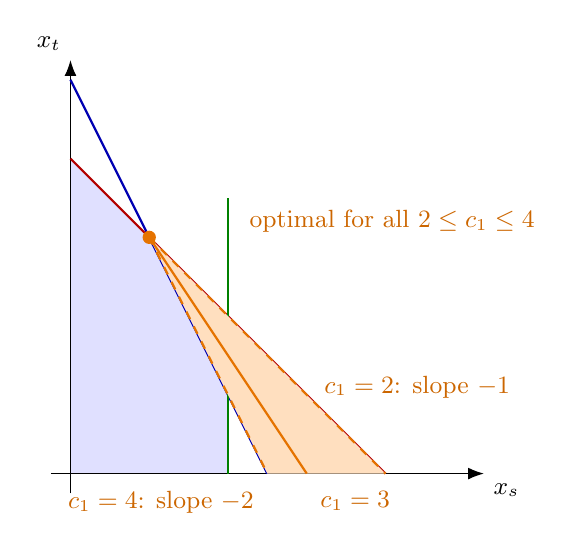
\begin{tikzpicture}[x=0.05cm, y=0.05cm, every node/.style={font=\small}, >={Latex[length=2mm]}]
	\fill[blue!12] (0,0) -- (40,0) -- (40,20) -- (20,60) -- (0,80) -- cycle;
	\draw[->] (-5,0) -- (105,0) node[below right] {$x_s$};
	\draw[->] (0,-5) -- (0,105) node[above left] {$x_t$};
	\draw[blue!70!black, thick] (50,0) -- (0,100);
	\draw[red!70!black, thick] (80,0) -- (0,80);
	\draw[green!50!black, thick] (40,0) -- (40,70);
	\fill[orange!25] (20,60) -- (80,0) -- (50,0) -- cycle;
	\draw[orange!90!black, thick, dashed] (20,60) -- (80,0);
	\draw[orange!90!black, thick, dashed] (20,60) -- (50,0);
	\draw[orange!90!black, thick] (20,60) -- (60,0);
	\node[orange!80!black, font=\small, anchor=west] at (62,22) {$c_1=2$: slope $-1$};
	\node[orange!80!black, font=\small, anchor=north east] at (49,-2) {$c_1=4$: slope $-2$};
	\node[orange!80!black, font=\small, anchor=north west] at (61,-2) {$c_1=3$};
	\fill[orange!90!black] (20,60) circle (2.4pt);
	\node[orange!80!black, font=\small, anchor=west] at (43,64) {optimal for all $2\le c_1\le4$};
	\end{tikzpicture}
\end{document}
